% Use the temporary template.
\documentclass{aer1315-pretty}

\usepackage{hyperref}
\usepackage{amsmath,amssymb}
\usepackage{eulervm}  % make math text non-italicized

% Author information
\author[]{ %
Christopher Ngigi\thanks{Graduate Research Assistant, Student ID: 999048230}\\
\textit{Institute for Aerospace Studies, University of Toronto}}

% Title
\title{Continuous Descent Approach: Benefits and Challenges}

% Abstract
 \abstract{ %
  This Interim Report investigates the effectiveness of Continuous Descent Approaches (CDA) which are part of Tailored Approaches (TA). Literature review of reports and publications indicating benefits of these are critiqued, and applicability as a whole analyzed. Findings from these sources are summarized.}


% Begin the document
\begin{document}
% Insert the title.
\maketitle

%%=======================================================================================================================
\section{Introduction}
While the aviation sector strives to reduce fuel consumption primarily for financial reasons, there is a growing awareness of its impact on the environment. We are still many years away from  resources being fully committed to the manufacture of breakthrough radical designs such as Blended Wing Bodies (BWB) which would significantly reduce the environmental footprint. These challenges stem from the expensive transition to new design procedures, since there is already a long-established and efficient interconnectivity that has been established by the major manufacturers with their subcontractors. Changes would potentially meet with certain resistance considering the high capital costs e.g. manufacturing equipment would need to be changed and replaced by an initially expensive process. Some of the newest entrants are utilizing new techniques to construct sections of aircraft fuselage such as the wings, tail sections and wing-box structures (i.e. the Boeing 787, Airbus A350, and Airbus A380). However, since these are still of conventional tube-and-wing configurations,  it is safe to say that it will be a long while  before any radical designs come into the market, and when they do, there may be the challenge of social acceptance.\par

Until this time arrives, we can try to improve the \textit{current} handling and operation of aircraft. We need to find techniques to alleviate the surging rise in fuel emissions, (particularly $CO_2$ - which has a potential life cycle of 200 years) due to the increasing popularity and need for air travel. How can we lower fuel consumption? Manufacturers have now began in earnest to use composite materials for some sections of aircraft fuselages, as mentioned above. Weight reductions have already been implemented by airline management to streamline efforts to reduce fuel consumption (financial motivation) - such as limiting the weight of checked luggage. Some airlines are implementing usage of Electronic Flight Bags (EFBs) in the cockpit as a weight-savings replacement to paper charts - Lufthansa even boasts of this on their website \cite{Lufty}. In terms of new materials and weight reduction, there is a current boom.\par

\begin{figure}
\centering
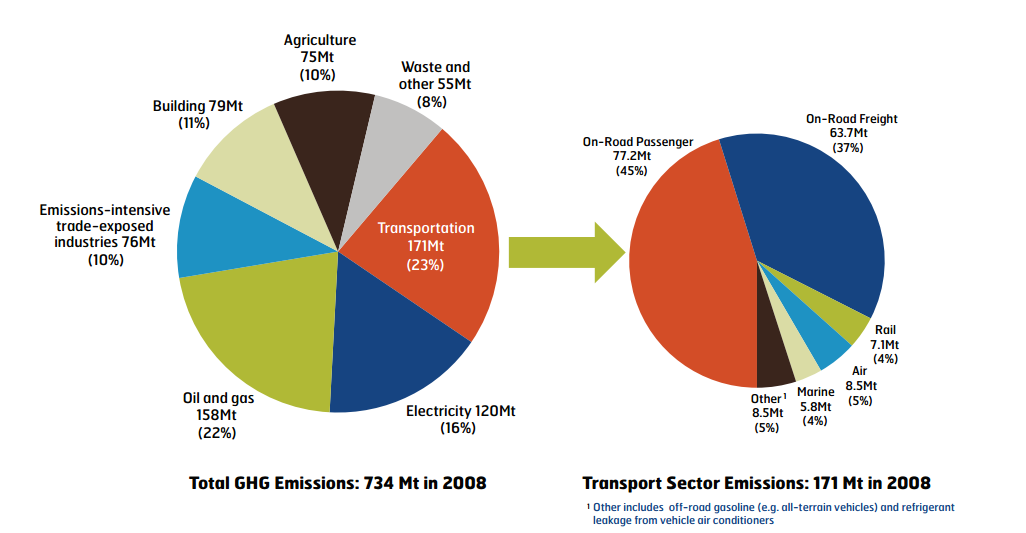
\includegraphics[height=0.42\textwidth]{figures/TotalEmissions.png}
	\caption{The Aviation Sector is responsible for approximately 5\% of emissions produced by the Transportation sector in Canada - Emissions from aviation data provided by Transport Canada. Source: \cite{TransportCanada}}	
	\label{fig:Emissions}
\end{figure}

\pagebreak[3]


%%--------------------------------------------------------------------------------------------
\goodbreak
\subsection{Pollution}

Presently, there is heavy emphasis on the control of pollution from the aviation sector, since it is a fast growing industry, projected to grow at an annual rate of 3-4\%. Data provided by Transport Canada \cite{TransportCanada} in figure \ref{fig:Emissions} shows that aviation is responsible for approximately 5\% of the entire transportation sector emissions (approximately 1\% of Canada's total greenhouse emissions).\par  

Engine manufacturers are continuously improving and refining engine design. An interesting observation is that there is current emphasis on reduction of $NO_x$ emissions. Within the engine, $NO_x$ formation occurs via the Zeldovich mechanism primarily in diffusion (non-premixed) type combustors. Diffusion type flames have a high primary zone temperature, which increases the production of thermal $NO_x$. The trend now is to implement partial-premixing, (i.e. mixing of air with fuel prior to entry into the combustion chamber, reducing the primary zone temperature, and consequently $NO_x$. However, the adverse effect is an increase $CO_2$ and Unburned Hydro Carbons (UHCs) emission. It is difficult to pit a pollutant against another, but based on time effects, $NO_x$ has a projected lifespan of approximately 2 weeks, while $CO_2$ nearly 200 years. $CO_2$ is a greenhouse gas that effectively raises the Earth's average temperature, and rather unfortunately, takes a very long time before it is re-absorbed.\par

Other pollutants such as $NO_x$, Aircraft Induced Cirrus are also harmful, however, $CO_2$ will be considered a principal target for emission reductions, in this day and age when global forest cover is reducing. The focus thus shifts to what can be currently done to reduce emissions from Aviation. Transport Canada have also shown projected reductions for $CO_2$ emissions in figure \ref{fig:CO2} and such reductions are effected by minimizing fuel burn.\par

\begin{figure}
\centering
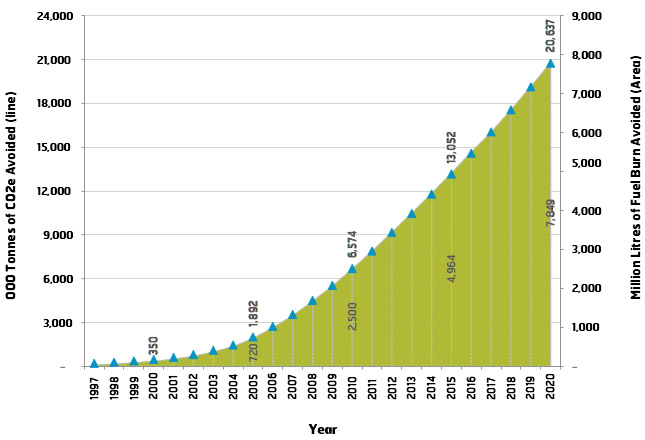
\includegraphics[height=0.4\textwidth]{figures/reduce_gas_emissions.jpg}%
	\caption{Historical and projected reductions in $CO_2$ Emissions as provided by Transport Canada. Source:  \cite{TransportCanada}}	
	\label{fig:CO2}
\end{figure}

Many governments have undertaken efforts to actively reduce aviation emission in a bid to control the surge in air travel movements, by modifying some of the standard practices. These could include allowing encouraging shorter taxi times at busy airports, charging airlines on Carbon Taxes, as well as regulatory bodies such as the Federal Aviation Administration regulating noise pollution.\par 
 

%%=====================================================================================================================
\section{Motivations for Continuous Descent Approach (CDA)}
\label{sec:CDA}
Continuous Descent Approach, applicable to the descent and approach phase of a flight, has been proposed as a technique for fuel reduction and noise abatement. This is achieved by modification of the Standard Arrival Route (STAR). The STAR is defined by ICAO as a standard Air Traffic Services (ATS) route identified in an approach procedure by which aircraft should proceed from the en-route phase to an initial approach fix. When close to this approach fix, the pilot typically receives vectoring from Air Traffic Control (ATC) to guide the aircraft to the initial waypoint of the ILS prior to landing. A comparison between the profiles of a CDA and a STAR are shown in figures \ref{fig:Compare} and \ref{fig:CompareYMML}. \par

The paper by Cao, Rathinam and Sun \cite{Cao:2011} describes CDA as a means to maintain the aircraft cruise altitude as much as can be achieved. This is highlighted in figure \ref{fig:KSFO ILS 28R} where a prolonged cruise altitude is depicted. When the aircraft reaches the top of descent (TOD), it begins to descend along a smooth slope (while the engines are running at idle or near-idle, thereby requiring significantly less engine thrust). When analysed in comparison to a conventional step-down descent, the CDA reduces fuel consumption, emission, and noise impact by avoiding "low" altitudes
(3,000 ft and 10,000 ft) level flight prior to interception of the 3 degree ILS Glideslope that is usually located 8 to 25 nautical miles away from the runway threshold. CDA also plays an important role in reducing flight time - this is because of the the longer duration high-altitude cruise with high speed. However, regardless of the environmental benefits, at the present moment CDA is yet to be ubiquitously implemented chiefly due to airport safety and efficiency concerns. Near idle throttle settings makes descent trajectories less predictable. As a result, air traffic controllers (ATCs) are required to reserve large sectors of airspace to separate any landing aircraft. Hence in contradictory fashion, this could lead to a significant reduction in the throughput (i.e. capacity for aircraft movements at an airport). So far, the CDA has been practiced only in low-traffic conditions or applied to a selected portion of inbound traffic in the off-peak hours (e.g. night time) rather than on a standard terminal airspace operation basis.\par 

When compared to a STandard Terminal ARrival (STAR) which has a typical staircase/cascade profile, the promises of CDA still show great potential. The STAR would require the aircraft to descend in segments along assigned way points, maintaining the regulated speed and altitude restrictions. This translates to flying at lower altitudes at lower speeds requiring early deployment of high-lift devices, and typically results in increased extra fuel-burn due to more power demand on the engines, as well as engine and airframe noise that would affect the surroundings near the airports.\par

\vspace{-0.8mm}
\begin{figure}[!h]
\centering
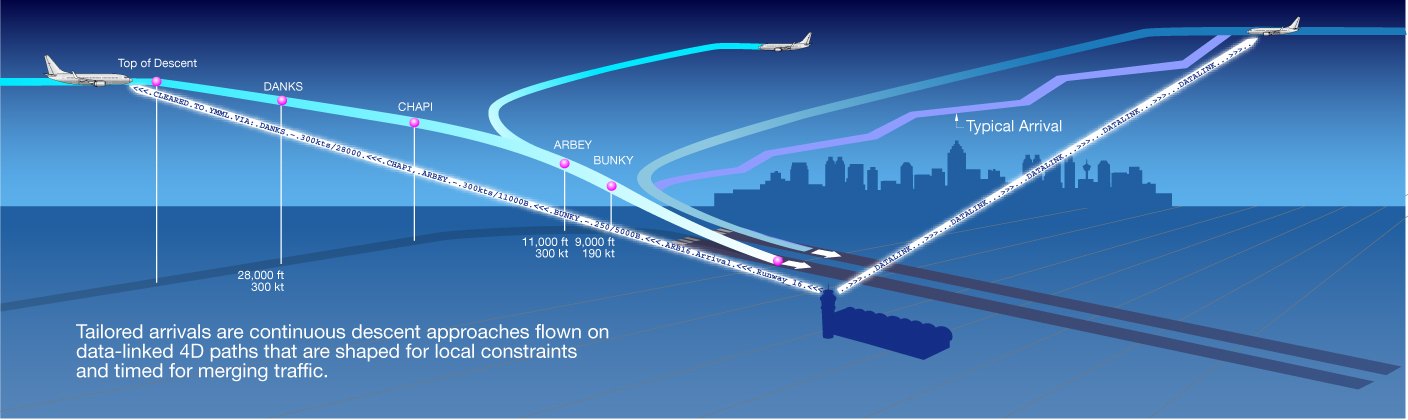
\includegraphics[width=1\textwidth]{figures/Tailored_Arrivals_YMML.jpg}
	\caption{Comparison of a STAR and TA profile at Melbourne International (YMML). Image Source: \cite{Boeing:a}}	
	\label{fig:CompareYMML}
\end{figure}
\vspace{-0.8mm}
In the mid-1970s, British Airways began constant angle descents into Heathrow Airport, from an initial height of 7000 ft above ground level, mainly aimed towards noise reduction. CDA has been developed to begin from the cruise altitude, enabling a smooth profiled descent into the airport. CDAs are part of the larger Tailored Approaches (TA), the term more commonly used in the USA.\par

\begin{figure}
\centering
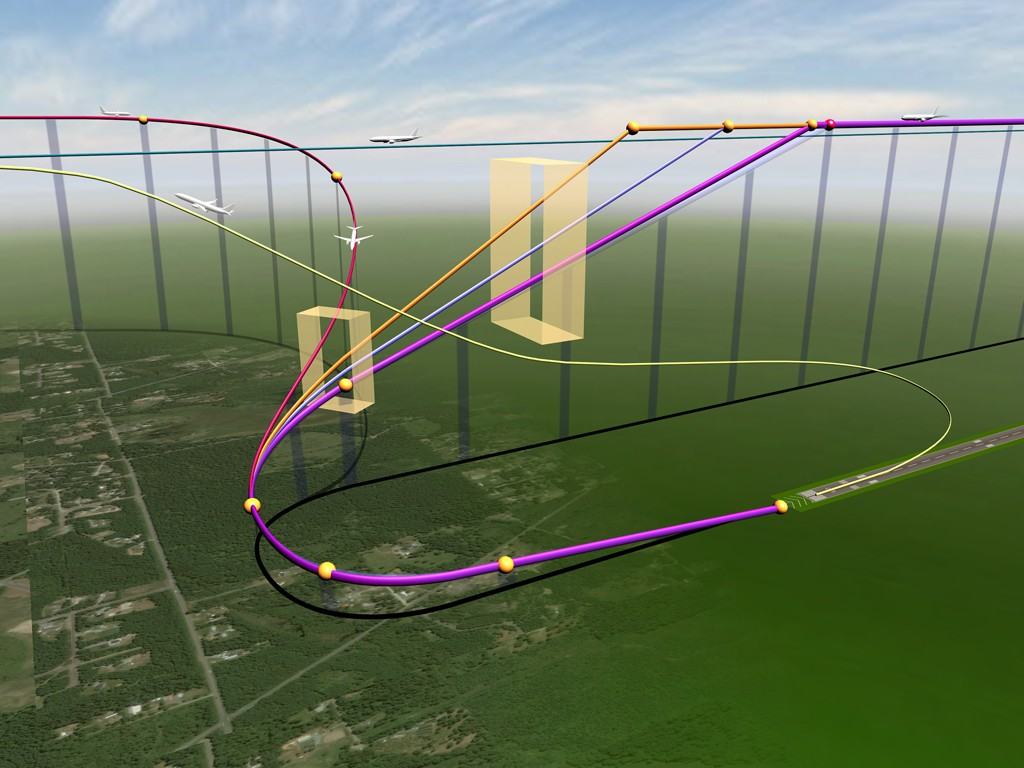
\includegraphics[width=0.45\textwidth]{figures/KSFO_CDA.png}
	\caption{A tailored approach into San Francisco International Airport (KSFO) Runway 28R. Image Source: \cite{Boeing}}	
	\label{fig:KSFO ILS 28R}
\end{figure}

Major Airports that have implemented the CDA/TA include:
\vspace{-2.4mm}
\begin{enumerate}
\itemsep-0.5em
\item Los Angeles International (KLAX)
\item Heathrow International (EGLL)
\item Hartsfield-Jackson International (KATL)
\item San Francisco International (KSFO)
\item Louisville International (KSDF)
\end{enumerate}
\vspace{-2.4mm}
Some of the benefits as reported by airlines that participated in the KATL study reported fuel savings of approximately 300-1000 pounds of fuel \cite{JP:a}. Since the CDA has a smooth glide profile, aircraft engines do not throttle up and down reducing the noise and emissions. Keeping engines at idle power can cut emissions of nitrogen oxides by nearly a third, and reduce noise along certain portions of the flight path prior to the Initial Fix point. CDA also has the benefit of being faster, saving a few minutes during the descent and landing phase of the flight.\par

Air New Zealand (ANZ) and QANTAS \cite{Copp:2007} participated in the Aspire program \cite{ANZ:a}, which aimed at having actual commercial flights that served as demonstrations  to set an ideal flight benchmark metric. On 12 September 2008 the inaugural test flight, an ANZ-operated Boeing 777, demonstrated the capabilities of the most advanced Air Navigation Services and airline fuel optimisation initiatives in current operation. This flight had all practical operational restraints removed: including air traffic congestion control vectoring, air traffic fixed route structure, procedures, flow restrictions and airline restraints. This flight had 3.5 tonnes fuel savings (11.2 tonnes $CO_2$ reduction). One month later Qantas flew a new A380 from KLAX -YMML saving 8.9 tonnes fuel (28 tonnes $CO_2$). Although idyllic, these flights served as a benchmark for achievable savings, to which CDA contributed. \par
%%===================================================================================================================
\section{Case Studies Summary}  \label{sec:case studies}

This report analyses the works of several researchers as listed out in the bibliography. In specifics:\par

The work of Park and Clarke \cite{Park:2015} analyzes some of the actual capabilities of CDA procedures. They build some computer models to investigate how various descent paths/trajectories can possibly impact the duration of a flight, as well as how much fuel would be consumed. For this purpose, they select profile data for a Boeing 737 and a Boeing 767 in their numerical study. After this, they compare the resulting optimized CDA trajectories to typical CDA trajectories that are currently used in CDA applications at several airports. (Clarke has a 2004 research paper on some preliminary CDA studies at Atlanta's Hartsfield-Jackson). They then proceed to divide the optimized CDA profile into two segments: cruise segment before the top of descent (TOD) and the descent segment from the TOD. Further, they split the descent section based on flap settings and speed restrictions. Flap settings affect the maximum speed attainable, and are also key contributors to noise emissions from the airframe.\par 

Cao et al \cite{Cao:2013} analyze CDA from a different perspective. Previous studies that had been done in this area did not always consider that using CDA will introduce uncertainties. The STAR technique is already an established routine, and predictions/controlling of multiple aircraft movements is easy. In CDA, however, the uncertainty is not guaranteed, and it is likely that to maintain aircraft spacing, more fuel could be used during descent, yet the CDA was intended to reduce fuel consumption. Their study then evaluates the fuel benefits of CDA at Atlanta Hartsfield-Jackson Airport (KATL) while considering potential flight time delays that result from conflict resolutions. Their fuel burn estimations are based on a corrected Thrust Specific Fuel Consumption (TSFC) model that is specifically designed for descent. They then determine potentially conflict-free CDAs in such a way that total arrival delays are minimized. Finally, resultant delays are converted to speed advisories that are communicated by ATC (or the equivalent method of maintaining the aircraft in a hold) during cruise phase to account for the impact of increased separations in CDAs. They then compare fuel consumption of CDA approach to that of real step-down trajectories which they obtained from KATL's radar database. \par


Jin and co-authors \cite{Jin:2013} decide to focus on the evaluation of the continuous-descent approach as a means to reduce fuel-consumption. Their research gives insights into the reasons why the CDA saves fuel, and they derive design guidelines for the useful procedures based on fuel burn (since this is heavily dependent on speed and altitude). They base this on the theoretical analysis that speed profile has a substantial impact just as important as altitude and attitude on the aircraft's fuel consumption as it approaches the landing phase. Finally they determine that the CDA is not an automatic fuel-saving procedure in itself: it rather depends on conformity to the speed schedule. Based on this model, the potential fuel savings due to the CDA at the San Francisco International Airport (KSFO) are estimated, and the accuracy of this estimation analysed. \par

Mur\c{c}a and M{\"u}ller \cite{Murca:2015} present an optimization approach that aims to reduce aircraft movement conflicts by enabling the dynamic scheduling of aircraft operations. This is very important to allow efficient management by supporting air traffic controllers. They are able to do this by calculating and implementing operationally feasible landing and departure times at an airport. They use a programming model which incorporates air route networks into the  air traffic control infrastructure and thereby allows effective ATC advisories for flight commands. It also goes an extra step by introducing alternative approach routes. Regarding the the computational running time, they obtained reasonable times to reach the optimal solution and eventually obtained delay reductions of up to $35 \%$ using comparisons from radar tracking database records from Sao Paulo/Guarulhos International Airport (SBGR). \par


Takeichi and Inami \cite{Takeichi:2010} discuss how arrival-times of CDA paths are determined by the top-of-descent and waypoint positions. (They define how controllable the arrival-time is  as being the difference between the fastest and the slowest arrival times.) They consider a tailored arrival path which is designed using the lowest number of track-to-fix and radius-to-fix legs neglecting the engine thrust. They proceed to investigate two types of tailored arrival paths; one which is determined by adjusting the waypoint positions with the fixed TOD, and the other being determined by TOD position with the fixed waypoints. They then analyse them to check if a set of appropriate boundary conditions both at the top of descent and landing are met, and they explore the behavior of the arrival-time difference from the standard continuous descent approach path using a representative set of inputs. Through several series of arrival-time analyses, they find that the tailored arrival paths determined by changing the waypoint positions can achieve the larger arrival-time controllability, (i.e. saving the most time) compared to those determined by changing the top-of-descent position. They finally suggest that it is possible to compose an arrival path with the maximum arrival-time controllability without increasing fuel consumption. \par

Turgut et al \cite{Enis:2010} analyze the impact of CDA on fuel consumption, noise and emissions. They model conventional and CDA procedures for a Boeing 757 in the Istanbul terminal area (TMA), which has five entry points (see figure \ref{IST}). Their model maintains actual speed and altitude limitations as boundary conditions at the Istanbul terminal area entry points. 

\begin{figure}
\centering
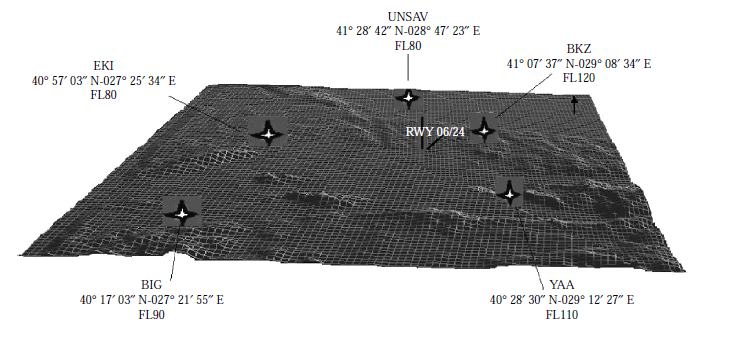
\includegraphics[height=0.45\textwidth]{figures/IST_terminal_area.png}
	\caption{Graphic showing layout of the Istanbul terminal area. Image Source: \cite{Enis:2010}}	
	\label{fig:IST}
\end{figure}

They found that for numerous approach cases, once the pilots had crossed the terminal area entry points, they would descend until minimum altitude limits and then continue to low-level altitudes until the Final Approach Point (FAP). Since this descent profile has a prolonged horizontal segment at lower altitude in its step-down approach, it necessitates more fuel consumption and flight duration compared to the CDA. They anticipate that the descent phase will contribute significant fuel saving potential and they use engine pressure ratio (EPR) readings to determine the engine thrust settings. Since the fuel consumption is a factor conditions such as weight, weather, traffic conditions, they program their model to various engine and airliner types. \par

Cao, Rathinam and Sun \cite{Cao:2011} present a rescheduling method for solving any potential conflicts between arriving aircraft flying along preferred descent paths using CDA. Their work is based on the 4-D trajectory concept: each aircraft will evaluate its own 4-D trajectory and the Estimated Time of Arrival (ETA) before initiating the descent procedure, and report these to ATC at the destination airport. These are in turn used by the ATC to sequence arriving aircraft. This potentially minimizes total delay while elimitating conflicting schedules for the the inbound traffic. Their computer model provides as a solution what they term as delay assignments. These are in turn used by the aircraft to adjust arrival times for conflict avoidance. ATC will impose necessary minimum separation between successive arrivals to meet the traffic movement capacity of the airport. Their proposed approach leads to a conflict-free inbound traffic, and more importantly, provides a means for CDA conflicts to be solved without changing the user-preferred trajectories, (hence CDA trajectories remain intact). \par

\begin{figure}[!h]
\centering
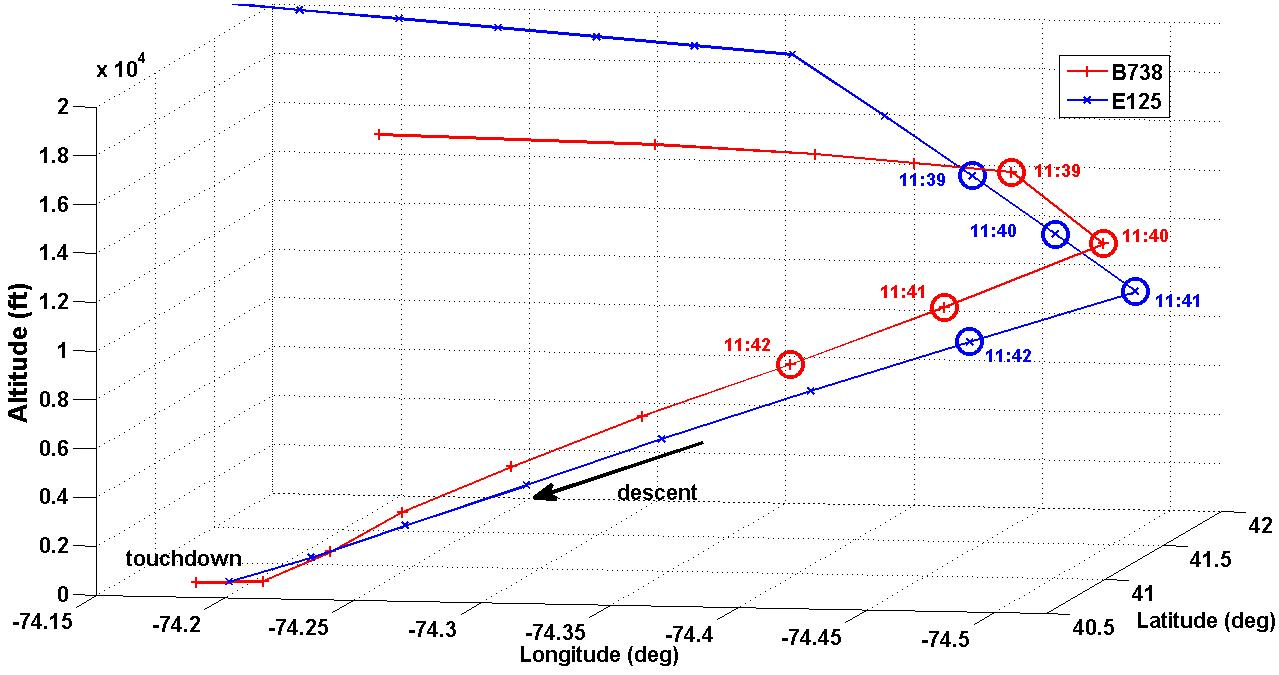
\includegraphics[height=0.4\textwidth]{figures/reschedule.jpg}
	\caption{Two aircraft in conflict get rescheduled. Image Source: \cite{Cao:2011}}	
	\label{fig:Rescheduled_Aircraft}
\end{figure}

Coppenbarger et al \cite{Copp:2007} discuss operational trials that were completed in January 2007 involving trans-Pacific flights into San Francisco during off-peak times. They describe how trajectory-based clearances were transmitted by data-link to Boeing 777 aircraft equipped with Future Air Navigation System avionics. NASA’s prototype ground-based automation Efficient Descent Advisor (EDA) software was  used for high-density arrival management and provided necessary clearances to accommodate some simulated metering constraints. \par

Robinson and Kamgarpur \cite{Rob:2010} estimate the potential benefits of continuous descents for more than $480,000$ flights to 25 major airports in the U.S. While they express their expectations for reductions in fuel consumption and greenhouse gas emissions,they mention that the benefits during periods of congestion are not well understood and need to be addressed. They proceed to construct some baseline trajectories  from flight plan and track data for flights arriving at some busy terminal areas and model two types of continuous descent trajectories: One enforcing a constant distance-to-fly constraint to simulate uncongested operations, while the other enforcing a constant time-to-fly constraint to simulate congested operations. They then calculated potential fuel savings for different continuous descent scenarios. \par

Nikoleris and co-authors \cite{Niko:2012} compare fuel consumption of alternative descent trajectories (from cruise altitude to meter fix) when required time of arrival is later than the nominal time of arrival at the meter fix. The required delay, which is essentially the difference between nominal and required times of arrival can be achieved by either slowing down the aircraft in the cruise and descent phases or flying a longer route at a constant altitude. They generate their results using performance models for ten different Boeing and Airbus aircraft obtained from Base of Aircraft Data. \par

Hayashi et al \cite{Hayashi:2011} propose an Efficient Descent Advisor (EDA) as a ground-based decision-support tool for Air Route Traffic Control Center (ARTCC) sector controllers for managing arrival flows. This work extends the research by Coppenbarger et al \cite{Copp:2010b}. Their tool calculates the manoeuvre instructions for an arrival flight to fly a conflict-free whenever possible and maintain high fuel-efficiency in a CDA while meeting a time restrictions at the Terminal Radar Approach Control (TRACON) boundary. In their paper they used speed variations and path-stretch maneuvers as the only degrees of freedom for the EDA software to find a solution. Their study further examined the feasibility of altitude change as an additional degree of freedom. \par

Alam and co-authors \cite{Alam:2010} investigate the benefits of CDA with change in traffic conditions and variable noise abatement rules and consider throughput capacity of transition airspace for multiple flights performing CDA operations. \par


Coppenbarger et al \cite{Copp:2010b} present an overview of development and testing of ground-based automation for accommodating fuel-efficient arrivals in heavy traffic. Their work serves as a foundation for Hayashi and co-workers\cite{Hayashi:2011}. They define the Efficient Descent Advisor (EDA), a decision-support tool for air-traffic controllers who managing arrival airspace in enroute facilities. The EDA tool allows a CDA and generates trajectory-based clearance advisories at low engine power while avoiding conflicts and maximizing arrival throughput at the airport. They use results from simulated pilot-ATC interaction to survey controller use and acceptance of EDA as a near-term capability for the Next-Generation Air Transportation System (NextGen) proposed in the U.S. \par


%%====================================================================================================================
\section{Results and Findings} \label{sec:results}

Park and Clarke \cite{Park:2015} 's results from the Boeing 737 study showed that if the aircraft flew along a minimum-fuel trajectory, savings of up to 54 kg of fuels can be achieved, representing $11.88\%$ of total fuel burn in the minimum-time case. (For a minimum-time trajectory, they manage to reduce flight time by 178 s, which is equivalent to a $12.16\%$ reduction in the flight time compared to the flight time needed for the minimum-fuel case). The CDA case results from their experiment are very similar to the results of the minimum-time case with a difference in fuel burn of only 5 kg and a flight-time difference of only 20 s. On the other hand in spite of the B767 having a larger size and weight, they observed the results to be very similar to those of the B737 when comparing the trajectories and speed profiles. The flight along the minimum-fuel profile consumed 85 kg less fuel than in the CDA case, which was an $11.7\%$ fuel savings when compared to the VNAV CDA case. The minimum-time profile is capable of reducing flight time by as much as 23 s when compared to the CDA case, and 161.32 s when compared to the minimum-fuel case.\par


Cao et al \cite{Cao:2013} got results that showed CDA does not guarantee fuel savings for individual arriving flights due to conflict avoidance. However, overall fuel consumption for all the aircraft at the airport is reduced. Removal of scheduling conflicts necessitated extra fuel consumption. They obtained mean value of the fuel savings of CDA with delays as 147.99 kg/flight while the mean value of the fuel savings of CDA without delays was 160.22 kg/flight. Delays resulted in  12.23 kg/flight reduction in the fuel savings on average, equivalent to $7.63\%$ of the savings attributed to the CDA vertical profiles. They found this estimation to be in accordance with Coppenbarger et al.\cite{Copp:2010b} where a 13.5 kg reduction of fuel savings per flight due to traffic was found, even though the absolute saving values may vary from 180 kg/flight to 2700 kg/flight. Once again, they observed that this was likely due to delays which may cause a decrease in the fuel savings. They observe that the CDA retains an almost constant descent gradient, hence fixing the vertical profiles a CDA flight can fly once a relevant speed profile depending on the type of aircraft 
is selected; corresponding to the fuel burn. Their trends of both the mean values indicated that savings were almost linearly correlated to the number of level flights executed. Finally, aircraft with long range flight segments showed the highest potential of savings. \par


Jin and co-authors \cite{Jin:2013} find that CDA saves fuel burn by eliminating level segments at low altitude (by elevating them to a high altitude); increasing average speed (most often, higher indicated airspeed is issued at higher altitudes); and, finally, The CDA moves the speed profile closer to the fuel-optimal speed profile. Their case study at San Francisco International Airport (KSFO) showed different results for varying speed profiles. 
They found that the speed from radar data was lower than the fuel-optimal speed, and consequently, higher altitude increased fuel consumption, resulting in the CDA consuming even more fuel. A faster speed profile would be required to reduce fuel consumption. Hence, to guarantee the CDA saves fuel, level-flight altitude must be elevated, and, perhaps more importantly, the the speed profile should be shifted closer to the fuel-optimal speed. Their findings reflected the notion that speed influences fuel consumption as significantly as, if not more than, altitude. They state that as much as 60 kg of fuel would be saved during a 10,000 m level segment at 9000 ft simply by changing the speed from 200 to 250 kt, and observe similar results in constant-speed descent. Finally, they state the conflict arising between fuel savings and noise reduction in the low-speed range. They find another reason why CDA saves fuel is that repeated engine throttling is largely avoided. \par

Mur\c{c}a and M{\"u}ller \cite{Murca:2015} find that the use of continuous decision variables actually increases the workload of ATC as well as that of the pilot, especially if a dynamic approach is used. They determine the controller to be responsible for determining the speed, altitude adjustment, and any other necessary manoeuvring required for each aircraft to reach the established fix. Should voice communications systems or other control actions be still necessary a broader underlying flow control conception is required. Moreover, since ATC is still responsible for implementing sequencing and scheduling, an optimization should incorporate such control problems. Their research has the objective to help the controller in determining the configuration of the STAR to be used and the number of holding procedures required. Such a configuration of the STAR could be selected standard procedures already validated by air traffic control bodies. \par

%%%%%%%%%%%%%%%% fix fix fix %%%%%%%%%%
Takeichi and Inami \cite{Takeichi:2010} use the equations of motion to analyze aircraft profiles while in the descent trajectory by analyzing the descent segments for a standard descent via a STAR, and comparing those to a CDA. They then use these equations to evaluate the expected arrival time for different flight angles. These flight angles involve a given approach at a certain angle towards the base leg approaching the runway. They then calculate fastest arrival times and paths that will enable this. \par
%%%%%%%%%%%%%%%%%%%%%%%%%%%%

Turgut et al \cite{Enis:2010}find that with implementation of CDA procedures, more than 40 kg fuel and 2 min time savings per flight are obtained;  7-9 percent of fuel savings were obtained. The largest savings were observed at entry point BIG as 44 kg, since this had the longest level flight distance as 55 nm. They found lowest fuel saving is obtained at YAA (see figure \ref{fig:IST}) as 27 kg for a level flight distance of 30.4 nm. Despite the fact that the level flight distance was directly proportional with the fuel burned, the other important factor is the percentage of how many miles were flown at relatively higher altitudes, and the latter would record higher fuel savings.  Effects of CDA on the flight duration reduction were between 17.8 and 19.3 percent by CDA, corresponding up to 2.8 min. This would amount to around 10 percent of the total descent duration.  Furthermore, they conclude that fuel savings are not only acquired from the reduction of the descent time, but also from the elevating level flight altitudes.\par


Cao, Rathinam and Sun \cite{Cao:2011} obtain simulation results in which their re-scheduling algorithm was able to de-conflict all the arriving aircraft with different prescribed horizontal separation settings in a full day terminal airspace operation at Newark Liberty International Airport (KEWR). The runtime of the algorithm was reasonable. A benefits analysis indicated savings of 80 tonnes of fuel and 638 minutes flight time if the step-down descents are changed to conflict-free CDAs over a 24 hour cycle. When compared to the conventional step-down approach, CDA reduced flight time and fuel consumption. As a trade-off, their statistical analysis obtained a total delay of 431 minutes was required for CDA separation. Such delay could be absorbed by delaying the aircraft either on the ground or while airborne. \par


Coppenbarger et al \cite{Copp:2007} found that for a Boeing 777 aircraft participating in the oceanic flights fuel savings of between 200 and 3,000 lbs per flight could be achieved (depending highly upon baseline traffic conditions) together with a corresponding reduction in $CO_2$ emissions of between 700 and 10,000 lbs per flight. Under light-congestion traffic conditions, results indicate average fuel savings of 242 lbs per flight while for medium and heavy traffic congestion scenarios, average estimated fuel savings increase to 358 lbs and 3,219 lbs per flight, respectively. They attribute the dramatic increase in estimated fuel savings for the heavy traffic comparison to the inefficiencies in their evaluation of a baseline scenario for achieving flow management and separation assurance under congested conditions. Such inefficiencies included an extra 30 nmi path-stretch segment performed in level flight at low altitude. Their results also suggested that idle-thrust, descent to the runway could reduce $CO_2$ emissions by 761 lbs per flight in comparison with B777 operations on similar routes conducted during light traffic congestion. In comparison with medium and heavy traffic-congestion baselines, CDA has the potential to reduce $CO_2$ emissions by as much as 1,128 lbs and 10,137 lbs per flight, respectively. \par


Robinson and Kamgarpur \cite{Rob:2010} found that estimated fuel savings was less than 25 kg for over $45\%$ of the flights, and less than 100 kg for over $87\%$ of the flights. The time-constrained trajectories showed $70-85\%$ less potential savings than the distance-constrained trajectories.  The terminal, transition, low en route and high en route level segments accounted for 62, 20, 8 and $10\%$ of the potential fuel savings, respectively.  The results for the partial continuous descent scenarios, whose level segments were replaced with level segments at the key altitudes instead of the cruise altitude, showed approximately half of the savings as the full continuous descent scenarios. This indicates that partial continuous descent scenarios (i.e., ones that initiate the continuous descent from higher intermediate altitudes instead of from cruise altitude) should be investigated as an alternative if a costly airspace redesign or infrastructure improvements must be avoided.They also found that  elimination of the level segments at intermediate altitudes decreased the flight time from top-of-descent to landing, because flights were able to maintain faster speeds at the higher altitudes. \par

\begin{figure}[!h]
\centering
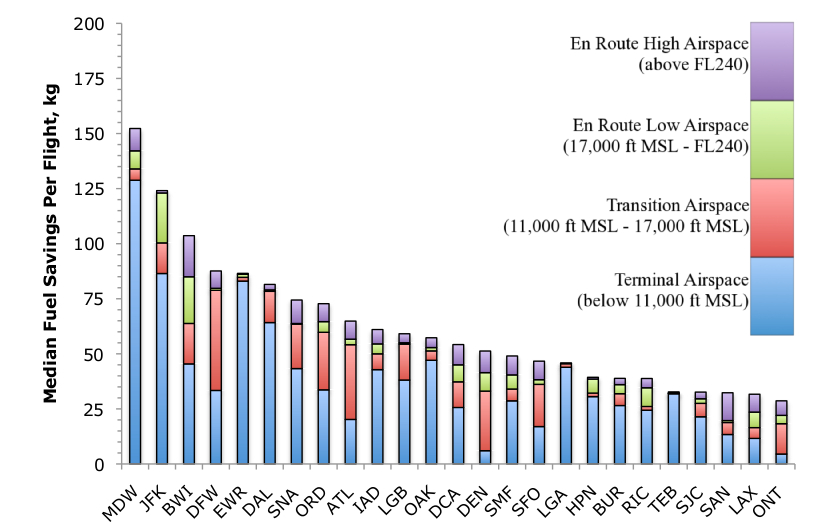
\includegraphics[height=0.4\textwidth]{figures/Comparison.jpg}
	\caption{Effect of continuous descent scenario on median fuel savings by airport. Source: \cite{Rob:2010}}	
	\label{fig:Compare}
\end{figure}

Nikoleris and co-authors \cite{Niko:2012} demonstrated that the most fuel-efficient speed control procedure for absorbing delay was by reducing descent speed as much as possible and then reducing cruise speed. They also show that for some aircraft, flying at a fixed flight path angle and constant airspeed resulted in lower fuel consumption compared to standard descents at idle-thrust and constant airspeed. Finally, they found that executing a path stretch maneuver at 35,000 feet altitude and continuing to descend at a reduced speed was more fuel efficient than inserting an intermediate-altitude cruise segment. When comparing the various type of idle-thrust descents for varying speeds, they obtain different results, namely:
\begin{itemize}
\item The  Idle-thrust Descent at Constant speed typically employed by pilots of large jets were found to be the most fuel efficient. Moreover, the descent-only procedure typically results in trajectories with lower fuel burn than the nominal trajectory. Aircraft thus spend more time on idle-thrust setting and less at higher cruise thrust compared to the nominal trajectory, resulting in lower fuel consumption. 
\item Constant Flight Path Angle Descent at Constant speed frequently executed by regional/business jets were examined for large commercial jets and were often found to yields lower fuel consumption than idle-thrust descent at constant Mach/CAS.
\item Idle-thrust Descent at Constant Flight Path Angle is not commonly executed, but it was found to result in lower fuel consumption than idle-thrust descent at constant speed in some instances. \par
\end{itemize}

\begin{figure}[!h]
\centering
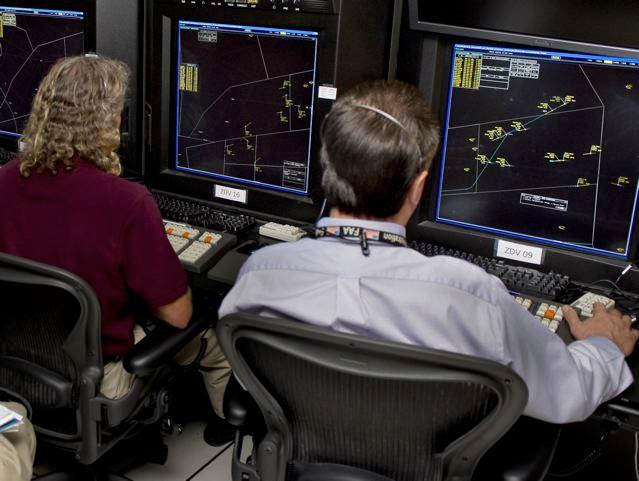
\includegraphics[width=0.6\textwidth]{figures/EDA.jpg}
	\caption{Efficient Descent Advisor (EDA), a decision-support tool for air-traffic controllers managing arrival airspace in enroute facilities. Image Source \cite{Copp:2010b}}	
	\label{fig:EDA}
\end{figure}


Hayashi et al \cite{Hayashi:2011} 's results of the human-in-the-loop simulation experiment (see figure \ref{fig:EDA} showed that the altitude-advisory capability reduced the number of conflicting EDA advisories. It also reduced controller workload when the traffic situation was complex. Results also suggested that changes to EDA’s user interface design and inter-sector coordination procedures are required for controllers to accept an altitude-advisory capability. They simulated some flights and found that some failed to meet time tolerances mainly because of manual controller intervention to adjust separation and pilots using the autopilot instead of the FMS to comply with speed clearance, essentially overriding the FMS optimized-path. \par


Alam and co-authors \cite{Alam:2010} found dynamic CDA approach led to reduction of $14.96\%$ in noise, $11.6\%$ reduction in NO x emission and $1.5\%$ reduction in fuel burn when compared to a standard CDA trajectory. They also suggested
routing and interval spacing to allow the system increase its throughput when congestion occurs. Regarding emissions biased traffic distribution showed highest emission for very dense scheduling, as it resulted in the highest frequency of hold patterns, leading to higher fuel burn and emission. However with increased inter arrival timings, emissions were significantly reduced. Corresponding trends were reflected in fuel burn. In terms of noise, biased traffic patterns remained the highest noise contributor, since more spiral routing patterns are required in the transition airspace to accommodate for the highly concentrated traffic in one area. \par


%========================================================================================

\section{Conclusions}  \label{sec:conclusion}

\begin{itemize}

\item Park and Clarke \cite{Park:2015}  show the following:
\begin{itemize}
\item CDAs can reduce operating costs by reducing the flight time, fuel burn, and reducing noise and gaseous emissions. 
\item The proposed VNAV CDA profiles have the possibility to be calculated by the aircraft's onboard FMS computer without additional equipment, they represent a practical implementation, while reducing required manual intervention. The study revealed that VNAV CDA profile performed nearly well as the optimal results. 
\item If the aircraft is capable of  quickly evaluating the parameter optimization using the proposed VNAV sequence, it becomes quite fast to calculate the optimal trajectory. If this is not the case, then it is possible to have a ground automation tool capable of solving the parameter-optimization problem using the proposed VNAV sequence, and then sending the calculated optimal parameter to the aircraft via data link. 
\item  To determine the optimal scheduling it is important for the ATC to be aware of individual aircraft performance envelopes, so as to have a good bearing on the acheivable time range of the CDA flight. 
\end{itemize}

\item Cao et al \cite{Cao:2013} help to evaluate  CDAs increased separation constraints to be able to factor in ATC control in estimation of the fuel savings benefits brought about by CDA. 
\begin{itemize}
\item They find that average fuel savings for each arrival flight is approximately 150kg/flight, which falls within limits of the IATA reported number 50~200 kg/flight. 
\item Although fuel savings for individual aircraft  may have been negative, macro-scale  airport wide evaluations indicate that CDA reduces fuel consumption. 
\item Due to delays, fuel savings drop by approximately 13 kg/flight and this was evaluated by an algorithm attempting to remove system conflicts.
\item They also found that increased separations led to a considerable impact on calculated flight delays. This essentially decreases airport throughput, and acts as a disadvantage of CDA.
\end{itemize}


\item Jin and co-authors \cite{Jin:2013} 
\begin{itemize}
\item The authors found that the case study at San Francisco International Airport (SFO) produced differing results on the proposed CDA techniques; i.e. analyzing aircraft arrival patterns and elevating priorities of some aircraft types over others.
\item Another observation was that fuel consumption in the terminal area was largely a function of the approach procedure, which specified the vertical and speed profiles. Fuel consumption increases with altitude and decreases with speed, while for high speeds, decreases with altitude and increases with speed. It is typical to find  fuel-optimal speed that minimizes fuel consumption for any given altitude.
\item By increasing cruise (or level flight) altitude as well as by increasing speed, the CDA typically reduces fuel consumption. This is highlighted by the observation that if a CDA procedure had a rather low speed profile, CDA would consume even more fuel than its conventional counterpart. It is crucial to design the speed profile in detail, just as is done for the vertical profile. 
\item The authors consider wide-body aircraft as the chief beneficiaries of the CDA design because their fuel consumption would be considerably reduced through well-designed CDA procedures, and the converse applies.
\item The authors believe that approach procedures of narrow-body aircraft can be sacrificed for optimized CDA procedures of wide-body aircraft and reach the rather alarming conclusion that CDA should be applied to wide-body aircraft, stating that CDA of narrow-body aircraft is neither favorable nor necessary. Considering the surge in air travel, narrow bodies should not be left out, since they account for majority of air traffic.
\end{itemize}



\item Mur\c{c}a and M{\"u}ller \cite{Murca:2015}

\begin{itemize}
\item Their model describes alternative arrival routes, and links arrival sequencing and scheduling to the Standard Terminal Arrival Routes and generates an output that can lead to directly executable flight commands. 
\item    They performed a real case study at SBGR analyze the performance of the model under different operating scenarios to test the model response time, as well as see how much reduction could be applied to potential delays.Their results showed reasonable computational times for obtaining the optimal solution within feasible computational times, as well as delay reductions of up to $35\%$ for the scenarios closest to the actual operations of SBGR. I
\end{itemize}


\item Turgut et al \cite{Enis:2010}

\begin{itemize}
\item For almost 35,000 flights, the fuel savings could be calculated as 1 M kg/year.
\item Savings for the other emission species such as NOx, CO and HC would have significant values as 24,500 kg for NOx, 2,625 kg for CO and 280 kg for HC corresponding to the fuel savings indicated.
\item The fuel savings by CDA procedures for a single airliner was obtained as ~44.3 kg. This was primarily by flying at higher altitude, (lowering drag). Time savings in the order of  of 2.8 min were estimated and were largely due to higher speeds.  
\item Traffic density is a big challenge to scheduling at peak times, and avaoidances must eb made to reduce ATC and pilot workload. Hence measures such as integrating an FMS to an optimization algorithm can deflect some of this workload.
\end{itemize}


\item Cao, Rathinam and Sun \cite{Cao:2011} 
\begin{itemize}
\item  To reduce conflict between aircraft flying the CDAs they separate the aircraft by rescheduling their expected times of arrival at the terminal aread boundary after imposing some minimum aircraft separation for safety purposes.
\item Their simulation results verified that potential conflicts could be resolved within an acceptable timeframe, thus allowing the airport to meet its throughput. They consider that their approach avoids tactical maneuvers which potentially disturb the CDA procedure. 
\end{itemize}


\item Coppenbarger et al \cite{Copp:2007} summarize their findings by  cconfirming that the San Francisco Oceanic Tailored Arrivals field trials demonstrated the ability to conduct highly efficient CDA operations under real-world conditions with commercial airplanes. Since the trials integrated air and ground automation via datalink they were an ideal proving ground to implement some of the foundations required to realize full NextGen capacity. To decongest the traffic conflicts during Tailored Arrivals, they used NASA’s ground-based EDA automation to customize trajectory solutions so that they could accommodate time-based metering constraints. 
Their results showed that errors in trajectory prediction could be significantly reduced by uplink of wind and descent speed data, although such performance in prediction can be achieved between air and ground automation. 
These results are important because accurate and compatible prediction performance between air and ground automation is fundamental to both the planning and execution of trajectory-based arrival operations. 
Based on real-world data that they gathered, they found substantial savings in fuel consumption, as well as significant reductions particularly when compared to standard approaches in heavy traffic. 


\item Robinson and Kamgarpur \cite{Rob:2010} 
\begin{itemize}
\item Found that estimated fuel savings were dependent on sample size and frequency (e.g., number of days, flights, etc.) and diversity (e.g., narrow-body to wide-body ratio, arrival routes, etc.) of the traffic samples analyzed.  In particular, they observed that aircraft of the "heavy" weight-class aircraft comprised $8\%$ of total operations, yet showed approximately $22\%$ of the predicted fuel savings.
\item However, eliminating level segments below 17,000 feet MSL did not have large impact on fuel savings. The duration of these level segments was less than 25 nmi for $52\%$ of the flights. Also, the level distance showed considerable variation between airports; only $16\%$ of SFO flights had level distances greater than 30 nmi, while $58\%$ of ORD flights did. 
It was more important to have full CDA from cruise altitude: Elimination of these level segments accounted for approximately $80\%$ of the fuel savings estimated. Furthermore, the estimated fuel savings was not distributed evenly among flights. It was less than 25 kg for more than $45\%$ of flights, and less than 100 kg for more than $87\%$ of the flights. As a result, $13\%$ of the flights accounted for $37\%$ of the total fuel savings.
\item The estimated fuel savings were not found to scale with traffic demand, since for large congestion, delays, re-routing and/or holds would be required. 
\item Enforcing a time constraint on CDA trajectories reduced estimated fuel savings by up to $70-85\%$. The reduction of potential benefits would be most severe when the delay required to be absorbed was the greatest.
\item Finally, CDA shows most benefit in reduction of fuel consumption when executed during periods of low to moderate traffic demand. 
\end{itemize}


\item Nikoleris and co-authors \cite{Niko:2012} 
\begin{itemize}
\item Four speed control techniques were considered for absorbing the delays needed for meeting the required time of arrival constraint at the meter fix with idle-thrust descent at constant airspeed, namely cruise-only, descent-only, cruise-first and descent-first. For a given range of delays, the descent-first method, was the most fuel efficient approach.
\item  Constant flight path angle descent at constant airspeed was found to be more fuel efficient compared to the standard descent procedure at idle-thrust and at constant airspeed. The difference in fuel consumption with these two procedures ranged between $-8\%$ and $+10\%$.
\item  The best approach to reduce fuel consumption would be to cruise at minimum speed, complete a path stretch at high altitude at that minimum speed, and then descend at minimum speed. This method is also utilized in the Efficient Descent Advisor (EDA) to generate advisories for meeting the required time of arrival.
\end{itemize}



\item Alam and co-authors \cite{Alam:2010} showed that a a dynamic CDA route could be developed to show any trade-off between the competing objectives of noise, emission and fuel burn. By assigning desired weights based on operational priority of each objective and using a simple search algorithm, the desired route can be selected for uplink to the aircraft's FMS. It is then possible to feed the waypoints into the FMS of the flight and autopilot can execute the CDA manoeuver.
Another benefit of dynamic CDA with cylindrical representation of transition airspace in rings, levels, and wedges is that it can be easily used for the distribution of aircraft noise in areas surrounding the airport. This can be achieved by blocking a set of wedge points that are to be avoided while generating the set of alternative routes from initial approach fix to final approach fix. 
Dynamic CDA trajectory is a step towards realization of 4D trajectory management in approach and descent phases of flight. Given the inherent uncertainties in air traffic environment and changing objectives of the ATCs, pre-published routes with fixed CDA altitude profiles may not be able to realize the full potential of CDA.
Such generated flexible CDA trajectories that are aircraft-specific and are optimized on given objectives (noise, fuel, emissions) and satisfy hard constraints of aircraft performance during descent and approach while meeting air traffic constraints (traffic, weather) can provide more efficient use of airspace and increase airport throughput capacity.


\item Coppenbarger et al \cite{Copp:2010b}  obtained very useful results from their human-in-the-loop experiments: primarily:

\begin{itemize}
\item Controller reaction was encouraging, suggesting that EDA has the potential to be implemented as a near-term capability with only minor changes to controller roles, responsibilities and procedures. 
\item Although EDA provides an obvious application for data link communications, simulations show that trajectory-based clearances involving speed and path can successfully be issued by voice. 
\item By providing controllers with a single, comprehensive arrival solution upstream, EDA was shown in simulation to reduce the number of required maneuver clearances by $70\%$, suggesting a significant potential reduction in controller and pilot workload.
\item Functions were added to allow controllers to quickly display trajectory information  including Top-of-Descent (TOD) to preserve situational awareness during trajectory-based operations in which airplanes are flying a variety of route, altitude and speed profiles.
\item Accurate ground-based trajectory prediction remains a key challenge for EDA implementation. Data collected during live traffic operations at Denver reveal that better predictions of TOD are required to implement EDA without procedurally sharing TOD information between controllers and pilots and/or increasing buffers for conflict avoidance in the vicinity of TOD. 
\end{itemize}

\end{itemize}

%%--------------------------------------------------------------------------------------------
\subsection{Key advantages} \label{ssec:comparisons}

\begin{itemize}
\item Fuel savings and emissions reductions\par
All authors agree on the fact that the CDA approach will lead to significant reductions in fuel consumptions as well as green house emissions. 
They mention the crucial role that the vertical and speed profile have on the effectiveness of fuel savings and  emissions reduction i.e. higher savings were realized for higher maintained altitudes provided the fuel-optimal speed profile was maintained. If the profiles are not optimum, then CDA could have worse performance than conventional step-down procedures. 

\item Time savings\par
Since majority of the flights maintained higher altitudes, they could maintain primarily faster cruise speeds with less speed restrictions, thus saving flight time. Delays would occur in the event that aircraft intervals were not maintained at the optimum spacing levels. Use of optimization software and introducing standard procedures by which either the pilots or the FMS/ground-based software could perform accurate calculations of optimal paths and expected times of arrival, then sequencing could be better performed and delays minimized.
\end{itemize}

%%--------------------------------------------------------------------------------------------
\subsection{Challenges} \label{ssec:challenges}

\begin{itemize}
\item Level of automation\par
Some of the above mentioned studies have described and shown the results of partial automation, by use of optimization software, much of the operator overload could be reduced, yet at the same time, it may prove in the near future that this system may have some faults that could pose safety risks, or even be very expensive to implement.

\item Flow of information\par
There will be a lot of information crossflow between ATC and the pilot/FMS via datalink, and this may cause a burdening on the system. While some authors have made reference to computer models that were developed or utilized during their study, this may not guarantee a successful, or effective implementation of the system to make sure the safety on the flight  and  ensure simplicity - it could easily occur that there

\item Traffic conditions\par
They also note that there is huge potential in implementing CDA at low-traffic conditions, and that extra emphasis need be placed on routing and scheduling techniques in the event of dense traffic times. This is important to realize the airport's throughput. It has been suggested that CDA  be carried out or implemented during off-peak conditions to minimize the strain on the airport throughput and ATC structure. It was also pointed out that although for individual aircraft, there were reports of negative fuel savings, the airport as a whole recorded significant savings, which, when viewed over a long time frame, would be a significant saving.
\end{itemize}

%%--------------------------------------------------------------------------------------------
\subsection{Suggested Implementation} \label{ssec:implementation}  

Some authors have pointed out the key savings made by wide-bodies that comprised the smaller percentage of aircraft traffic, yet reported significant savings on fuel consumption, and the same could be said about the aircraft that maintained high-elevation altitude segments prior to descent.\par

Since there is an increase in air travel, and this is particularly the case for regional flights, it is believed that narrow-bodies should be also part of the main focus, since they comprise majority of air traffic. If a system could be put into place to schedule and space out the aircraft as they arrive, then exponential savings could be made.\par

Hence, based on the literature review, it has been shown that CDA offers a big potential, and a temporary reprieve, while emerging technology and alternative energy sources are on the drawing boards.

                       
%%===================================================================================================================



%%=====================================================================================================================
\section*{Acknowledgements}
This document template was prepared by Derek Dalle with help from Sara Spangelo and was obtained from \url{http://www-personal.umich.edu/~dalle/codes/aiaa-pretty/downloads/}  

% References
%\nocite{*}
\bibliographystyle{aiaa}
\bibliography{./bib/chris}


\end{document}
